
% Default to the notebook output style

    


% Inherit from the specified cell style.




    
\documentclass[11pt]{article}

    
    
    \usepackage[T1]{fontenc}
    % Nicer default font (+ math font) than Computer Modern for most use cases
    \usepackage{mathpazo}

    % Basic figure setup, for now with no caption control since it's done
    % automatically by Pandoc (which extracts ![](path) syntax from Markdown).
    \usepackage{graphicx}
    % We will generate all images so they have a width \maxwidth. This means
    % that they will get their normal width if they fit onto the page, but
    % are scaled down if they would overflow the margins.
    \makeatletter
    \def\maxwidth{\ifdim\Gin@nat@width>\linewidth\linewidth
    \else\Gin@nat@width\fi}
    \makeatother
    \let\Oldincludegraphics\includegraphics
    % Set max figure width to be 80% of text width, for now hardcoded.
    \renewcommand{\includegraphics}[1]{\Oldincludegraphics[width=.8\maxwidth]{#1}}
    % Ensure that by default, figures have no caption (until we provide a
    % proper Figure object with a Caption API and a way to capture that
    % in the conversion process - todo).
    \usepackage{caption}
    \DeclareCaptionLabelFormat{nolabel}{}
    \captionsetup{labelformat=nolabel}

    \usepackage{adjustbox} % Used to constrain images to a maximum size 
    \usepackage{xcolor} % Allow colors to be defined
    \usepackage{enumerate} % Needed for markdown enumerations to work
    \usepackage{geometry} % Used to adjust the document margins
    \usepackage{amsmath} % Equations
    \usepackage{amssymb} % Equations
    \usepackage{textcomp} % defines textquotesingle
    % Hack from http://tex.stackexchange.com/a/47451/13684:
    \AtBeginDocument{%
        \def\PYZsq{\textquotesingle}% Upright quotes in Pygmentized code
    }
    \usepackage{upquote} % Upright quotes for verbatim code
    \usepackage{eurosym} % defines \euro
    \usepackage[mathletters]{ucs} % Extended unicode (utf-8) support
    \usepackage[utf8x]{inputenc} % Allow utf-8 characters in the tex document
    \usepackage{fancyvrb} % verbatim replacement that allows latex
    \usepackage{grffile} % extends the file name processing of package graphics 
                         % to support a larger range 
    % The hyperref package gives us a pdf with properly built
    % internal navigation ('pdf bookmarks' for the table of contents,
    % internal cross-reference links, web links for URLs, etc.)
    \usepackage{hyperref}
    \usepackage{longtable} % longtable support required by pandoc >1.10
    \usepackage{booktabs}  % table support for pandoc > 1.12.2
    \usepackage[inline]{enumitem} % IRkernel/repr support (it uses the enumerate* environment)
    \usepackage[normalem]{ulem} % ulem is needed to support strikethroughs (\sout)
                                % normalem makes italics be italics, not underlines
    

    
    
    % Colors for the hyperref package
    \definecolor{urlcolor}{rgb}{0,.145,.698}
    \definecolor{linkcolor}{rgb}{.71,0.21,0.01}
    \definecolor{citecolor}{rgb}{.12,.54,.11}

    % ANSI colors
    \definecolor{ansi-black}{HTML}{3E424D}
    \definecolor{ansi-black-intense}{HTML}{282C36}
    \definecolor{ansi-red}{HTML}{E75C58}
    \definecolor{ansi-red-intense}{HTML}{B22B31}
    \definecolor{ansi-green}{HTML}{00A250}
    \definecolor{ansi-green-intense}{HTML}{007427}
    \definecolor{ansi-yellow}{HTML}{DDB62B}
    \definecolor{ansi-yellow-intense}{HTML}{B27D12}
    \definecolor{ansi-blue}{HTML}{208FFB}
    \definecolor{ansi-blue-intense}{HTML}{0065CA}
    \definecolor{ansi-magenta}{HTML}{D160C4}
    \definecolor{ansi-magenta-intense}{HTML}{A03196}
    \definecolor{ansi-cyan}{HTML}{60C6C8}
    \definecolor{ansi-cyan-intense}{HTML}{258F8F}
    \definecolor{ansi-white}{HTML}{C5C1B4}
    \definecolor{ansi-white-intense}{HTML}{A1A6B2}

    % commands and environments needed by pandoc snippets
    % extracted from the output of `pandoc -s`
    \providecommand{\tightlist}{%
      \setlength{\itemsep}{0pt}\setlength{\parskip}{0pt}}
    \DefineVerbatimEnvironment{Highlighting}{Verbatim}{commandchars=\\\{\}}
    % Add ',fontsize=\small' for more characters per line
    \newenvironment{Shaded}{}{}
    \newcommand{\KeywordTok}[1]{\textcolor[rgb]{0.00,0.44,0.13}{\textbf{{#1}}}}
    \newcommand{\DataTypeTok}[1]{\textcolor[rgb]{0.56,0.13,0.00}{{#1}}}
    \newcommand{\DecValTok}[1]{\textcolor[rgb]{0.25,0.63,0.44}{{#1}}}
    \newcommand{\BaseNTok}[1]{\textcolor[rgb]{0.25,0.63,0.44}{{#1}}}
    \newcommand{\FloatTok}[1]{\textcolor[rgb]{0.25,0.63,0.44}{{#1}}}
    \newcommand{\CharTok}[1]{\textcolor[rgb]{0.25,0.44,0.63}{{#1}}}
    \newcommand{\StringTok}[1]{\textcolor[rgb]{0.25,0.44,0.63}{{#1}}}
    \newcommand{\CommentTok}[1]{\textcolor[rgb]{0.38,0.63,0.69}{\textit{{#1}}}}
    \newcommand{\OtherTok}[1]{\textcolor[rgb]{0.00,0.44,0.13}{{#1}}}
    \newcommand{\AlertTok}[1]{\textcolor[rgb]{1.00,0.00,0.00}{\textbf{{#1}}}}
    \newcommand{\FunctionTok}[1]{\textcolor[rgb]{0.02,0.16,0.49}{{#1}}}
    \newcommand{\RegionMarkerTok}[1]{{#1}}
    \newcommand{\ErrorTok}[1]{\textcolor[rgb]{1.00,0.00,0.00}{\textbf{{#1}}}}
    \newcommand{\NormalTok}[1]{{#1}}
    
    % Additional commands for more recent versions of Pandoc
    \newcommand{\ConstantTok}[1]{\textcolor[rgb]{0.53,0.00,0.00}{{#1}}}
    \newcommand{\SpecialCharTok}[1]{\textcolor[rgb]{0.25,0.44,0.63}{{#1}}}
    \newcommand{\VerbatimStringTok}[1]{\textcolor[rgb]{0.25,0.44,0.63}{{#1}}}
    \newcommand{\SpecialStringTok}[1]{\textcolor[rgb]{0.73,0.40,0.53}{{#1}}}
    \newcommand{\ImportTok}[1]{{#1}}
    \newcommand{\DocumentationTok}[1]{\textcolor[rgb]{0.73,0.13,0.13}{\textit{{#1}}}}
    \newcommand{\AnnotationTok}[1]{\textcolor[rgb]{0.38,0.63,0.69}{\textbf{\textit{{#1}}}}}
    \newcommand{\CommentVarTok}[1]{\textcolor[rgb]{0.38,0.63,0.69}{\textbf{\textit{{#1}}}}}
    \newcommand{\VariableTok}[1]{\textcolor[rgb]{0.10,0.09,0.49}{{#1}}}
    \newcommand{\ControlFlowTok}[1]{\textcolor[rgb]{0.00,0.44,0.13}{\textbf{{#1}}}}
    \newcommand{\OperatorTok}[1]{\textcolor[rgb]{0.40,0.40,0.40}{{#1}}}
    \newcommand{\BuiltInTok}[1]{{#1}}
    \newcommand{\ExtensionTok}[1]{{#1}}
    \newcommand{\PreprocessorTok}[1]{\textcolor[rgb]{0.74,0.48,0.00}{{#1}}}
    \newcommand{\AttributeTok}[1]{\textcolor[rgb]{0.49,0.56,0.16}{{#1}}}
    \newcommand{\InformationTok}[1]{\textcolor[rgb]{0.38,0.63,0.69}{\textbf{\textit{{#1}}}}}
    \newcommand{\WarningTok}[1]{\textcolor[rgb]{0.38,0.63,0.69}{\textbf{\textit{{#1}}}}}
    
    
    % Define a nice break command that doesn't care if a line doesn't already
    % exist.
    \def\br{\hspace*{\fill} \\* }
    % Math Jax compatability definitions
    \def\gt{>}
    \def\lt{<}
    % Document parameters
    \title{hw3}
    
    
    

    % Pygments definitions
    
\makeatletter
\def\PY@reset{\let\PY@it=\relax \let\PY@bf=\relax%
    \let\PY@ul=\relax \let\PY@tc=\relax%
    \let\PY@bc=\relax \let\PY@ff=\relax}
\def\PY@tok#1{\csname PY@tok@#1\endcsname}
\def\PY@toks#1+{\ifx\relax#1\empty\else%
    \PY@tok{#1}\expandafter\PY@toks\fi}
\def\PY@do#1{\PY@bc{\PY@tc{\PY@ul{%
    \PY@it{\PY@bf{\PY@ff{#1}}}}}}}
\def\PY#1#2{\PY@reset\PY@toks#1+\relax+\PY@do{#2}}

\expandafter\def\csname PY@tok@w\endcsname{\def\PY@tc##1{\textcolor[rgb]{0.73,0.73,0.73}{##1}}}
\expandafter\def\csname PY@tok@c\endcsname{\let\PY@it=\textit\def\PY@tc##1{\textcolor[rgb]{0.25,0.50,0.50}{##1}}}
\expandafter\def\csname PY@tok@cp\endcsname{\def\PY@tc##1{\textcolor[rgb]{0.74,0.48,0.00}{##1}}}
\expandafter\def\csname PY@tok@k\endcsname{\let\PY@bf=\textbf\def\PY@tc##1{\textcolor[rgb]{0.00,0.50,0.00}{##1}}}
\expandafter\def\csname PY@tok@kp\endcsname{\def\PY@tc##1{\textcolor[rgb]{0.00,0.50,0.00}{##1}}}
\expandafter\def\csname PY@tok@kt\endcsname{\def\PY@tc##1{\textcolor[rgb]{0.69,0.00,0.25}{##1}}}
\expandafter\def\csname PY@tok@o\endcsname{\def\PY@tc##1{\textcolor[rgb]{0.40,0.40,0.40}{##1}}}
\expandafter\def\csname PY@tok@ow\endcsname{\let\PY@bf=\textbf\def\PY@tc##1{\textcolor[rgb]{0.67,0.13,1.00}{##1}}}
\expandafter\def\csname PY@tok@nb\endcsname{\def\PY@tc##1{\textcolor[rgb]{0.00,0.50,0.00}{##1}}}
\expandafter\def\csname PY@tok@nf\endcsname{\def\PY@tc##1{\textcolor[rgb]{0.00,0.00,1.00}{##1}}}
\expandafter\def\csname PY@tok@nc\endcsname{\let\PY@bf=\textbf\def\PY@tc##1{\textcolor[rgb]{0.00,0.00,1.00}{##1}}}
\expandafter\def\csname PY@tok@nn\endcsname{\let\PY@bf=\textbf\def\PY@tc##1{\textcolor[rgb]{0.00,0.00,1.00}{##1}}}
\expandafter\def\csname PY@tok@ne\endcsname{\let\PY@bf=\textbf\def\PY@tc##1{\textcolor[rgb]{0.82,0.25,0.23}{##1}}}
\expandafter\def\csname PY@tok@nv\endcsname{\def\PY@tc##1{\textcolor[rgb]{0.10,0.09,0.49}{##1}}}
\expandafter\def\csname PY@tok@no\endcsname{\def\PY@tc##1{\textcolor[rgb]{0.53,0.00,0.00}{##1}}}
\expandafter\def\csname PY@tok@nl\endcsname{\def\PY@tc##1{\textcolor[rgb]{0.63,0.63,0.00}{##1}}}
\expandafter\def\csname PY@tok@ni\endcsname{\let\PY@bf=\textbf\def\PY@tc##1{\textcolor[rgb]{0.60,0.60,0.60}{##1}}}
\expandafter\def\csname PY@tok@na\endcsname{\def\PY@tc##1{\textcolor[rgb]{0.49,0.56,0.16}{##1}}}
\expandafter\def\csname PY@tok@nt\endcsname{\let\PY@bf=\textbf\def\PY@tc##1{\textcolor[rgb]{0.00,0.50,0.00}{##1}}}
\expandafter\def\csname PY@tok@nd\endcsname{\def\PY@tc##1{\textcolor[rgb]{0.67,0.13,1.00}{##1}}}
\expandafter\def\csname PY@tok@s\endcsname{\def\PY@tc##1{\textcolor[rgb]{0.73,0.13,0.13}{##1}}}
\expandafter\def\csname PY@tok@sd\endcsname{\let\PY@it=\textit\def\PY@tc##1{\textcolor[rgb]{0.73,0.13,0.13}{##1}}}
\expandafter\def\csname PY@tok@si\endcsname{\let\PY@bf=\textbf\def\PY@tc##1{\textcolor[rgb]{0.73,0.40,0.53}{##1}}}
\expandafter\def\csname PY@tok@se\endcsname{\let\PY@bf=\textbf\def\PY@tc##1{\textcolor[rgb]{0.73,0.40,0.13}{##1}}}
\expandafter\def\csname PY@tok@sr\endcsname{\def\PY@tc##1{\textcolor[rgb]{0.73,0.40,0.53}{##1}}}
\expandafter\def\csname PY@tok@ss\endcsname{\def\PY@tc##1{\textcolor[rgb]{0.10,0.09,0.49}{##1}}}
\expandafter\def\csname PY@tok@sx\endcsname{\def\PY@tc##1{\textcolor[rgb]{0.00,0.50,0.00}{##1}}}
\expandafter\def\csname PY@tok@m\endcsname{\def\PY@tc##1{\textcolor[rgb]{0.40,0.40,0.40}{##1}}}
\expandafter\def\csname PY@tok@gh\endcsname{\let\PY@bf=\textbf\def\PY@tc##1{\textcolor[rgb]{0.00,0.00,0.50}{##1}}}
\expandafter\def\csname PY@tok@gu\endcsname{\let\PY@bf=\textbf\def\PY@tc##1{\textcolor[rgb]{0.50,0.00,0.50}{##1}}}
\expandafter\def\csname PY@tok@gd\endcsname{\def\PY@tc##1{\textcolor[rgb]{0.63,0.00,0.00}{##1}}}
\expandafter\def\csname PY@tok@gi\endcsname{\def\PY@tc##1{\textcolor[rgb]{0.00,0.63,0.00}{##1}}}
\expandafter\def\csname PY@tok@gr\endcsname{\def\PY@tc##1{\textcolor[rgb]{1.00,0.00,0.00}{##1}}}
\expandafter\def\csname PY@tok@ge\endcsname{\let\PY@it=\textit}
\expandafter\def\csname PY@tok@gs\endcsname{\let\PY@bf=\textbf}
\expandafter\def\csname PY@tok@gp\endcsname{\let\PY@bf=\textbf\def\PY@tc##1{\textcolor[rgb]{0.00,0.00,0.50}{##1}}}
\expandafter\def\csname PY@tok@go\endcsname{\def\PY@tc##1{\textcolor[rgb]{0.53,0.53,0.53}{##1}}}
\expandafter\def\csname PY@tok@gt\endcsname{\def\PY@tc##1{\textcolor[rgb]{0.00,0.27,0.87}{##1}}}
\expandafter\def\csname PY@tok@err\endcsname{\def\PY@bc##1{\setlength{\fboxsep}{0pt}\fcolorbox[rgb]{1.00,0.00,0.00}{1,1,1}{\strut ##1}}}
\expandafter\def\csname PY@tok@kc\endcsname{\let\PY@bf=\textbf\def\PY@tc##1{\textcolor[rgb]{0.00,0.50,0.00}{##1}}}
\expandafter\def\csname PY@tok@kd\endcsname{\let\PY@bf=\textbf\def\PY@tc##1{\textcolor[rgb]{0.00,0.50,0.00}{##1}}}
\expandafter\def\csname PY@tok@kn\endcsname{\let\PY@bf=\textbf\def\PY@tc##1{\textcolor[rgb]{0.00,0.50,0.00}{##1}}}
\expandafter\def\csname PY@tok@kr\endcsname{\let\PY@bf=\textbf\def\PY@tc##1{\textcolor[rgb]{0.00,0.50,0.00}{##1}}}
\expandafter\def\csname PY@tok@bp\endcsname{\def\PY@tc##1{\textcolor[rgb]{0.00,0.50,0.00}{##1}}}
\expandafter\def\csname PY@tok@fm\endcsname{\def\PY@tc##1{\textcolor[rgb]{0.00,0.00,1.00}{##1}}}
\expandafter\def\csname PY@tok@vc\endcsname{\def\PY@tc##1{\textcolor[rgb]{0.10,0.09,0.49}{##1}}}
\expandafter\def\csname PY@tok@vg\endcsname{\def\PY@tc##1{\textcolor[rgb]{0.10,0.09,0.49}{##1}}}
\expandafter\def\csname PY@tok@vi\endcsname{\def\PY@tc##1{\textcolor[rgb]{0.10,0.09,0.49}{##1}}}
\expandafter\def\csname PY@tok@vm\endcsname{\def\PY@tc##1{\textcolor[rgb]{0.10,0.09,0.49}{##1}}}
\expandafter\def\csname PY@tok@sa\endcsname{\def\PY@tc##1{\textcolor[rgb]{0.73,0.13,0.13}{##1}}}
\expandafter\def\csname PY@tok@sb\endcsname{\def\PY@tc##1{\textcolor[rgb]{0.73,0.13,0.13}{##1}}}
\expandafter\def\csname PY@tok@sc\endcsname{\def\PY@tc##1{\textcolor[rgb]{0.73,0.13,0.13}{##1}}}
\expandafter\def\csname PY@tok@dl\endcsname{\def\PY@tc##1{\textcolor[rgb]{0.73,0.13,0.13}{##1}}}
\expandafter\def\csname PY@tok@s2\endcsname{\def\PY@tc##1{\textcolor[rgb]{0.73,0.13,0.13}{##1}}}
\expandafter\def\csname PY@tok@sh\endcsname{\def\PY@tc##1{\textcolor[rgb]{0.73,0.13,0.13}{##1}}}
\expandafter\def\csname PY@tok@s1\endcsname{\def\PY@tc##1{\textcolor[rgb]{0.73,0.13,0.13}{##1}}}
\expandafter\def\csname PY@tok@mb\endcsname{\def\PY@tc##1{\textcolor[rgb]{0.40,0.40,0.40}{##1}}}
\expandafter\def\csname PY@tok@mf\endcsname{\def\PY@tc##1{\textcolor[rgb]{0.40,0.40,0.40}{##1}}}
\expandafter\def\csname PY@tok@mh\endcsname{\def\PY@tc##1{\textcolor[rgb]{0.40,0.40,0.40}{##1}}}
\expandafter\def\csname PY@tok@mi\endcsname{\def\PY@tc##1{\textcolor[rgb]{0.40,0.40,0.40}{##1}}}
\expandafter\def\csname PY@tok@il\endcsname{\def\PY@tc##1{\textcolor[rgb]{0.40,0.40,0.40}{##1}}}
\expandafter\def\csname PY@tok@mo\endcsname{\def\PY@tc##1{\textcolor[rgb]{0.40,0.40,0.40}{##1}}}
\expandafter\def\csname PY@tok@ch\endcsname{\let\PY@it=\textit\def\PY@tc##1{\textcolor[rgb]{0.25,0.50,0.50}{##1}}}
\expandafter\def\csname PY@tok@cm\endcsname{\let\PY@it=\textit\def\PY@tc##1{\textcolor[rgb]{0.25,0.50,0.50}{##1}}}
\expandafter\def\csname PY@tok@cpf\endcsname{\let\PY@it=\textit\def\PY@tc##1{\textcolor[rgb]{0.25,0.50,0.50}{##1}}}
\expandafter\def\csname PY@tok@c1\endcsname{\let\PY@it=\textit\def\PY@tc##1{\textcolor[rgb]{0.25,0.50,0.50}{##1}}}
\expandafter\def\csname PY@tok@cs\endcsname{\let\PY@it=\textit\def\PY@tc##1{\textcolor[rgb]{0.25,0.50,0.50}{##1}}}

\def\PYZbs{\char`\\}
\def\PYZus{\char`\_}
\def\PYZob{\char`\{}
\def\PYZcb{\char`\}}
\def\PYZca{\char`\^}
\def\PYZam{\char`\&}
\def\PYZlt{\char`\<}
\def\PYZgt{\char`\>}
\def\PYZsh{\char`\#}
\def\PYZpc{\char`\%}
\def\PYZdl{\char`\$}
\def\PYZhy{\char`\-}
\def\PYZsq{\char`\'}
\def\PYZdq{\char`\"}
\def\PYZti{\char`\~}
% for compatibility with earlier versions
\def\PYZat{@}
\def\PYZlb{[}
\def\PYZrb{]}
\makeatother


    % Exact colors from NB
    \definecolor{incolor}{rgb}{0.0, 0.0, 0.5}
    \definecolor{outcolor}{rgb}{0.545, 0.0, 0.0}



    
    % Prevent overflowing lines due to hard-to-break entities
    \sloppy 
    % Setup hyperref package
    \hypersetup{
      breaklinks=true,  % so long urls are correctly broken across lines
      colorlinks=true,
      urlcolor=urlcolor,
      linkcolor=linkcolor,
      citecolor=citecolor,
      }
    % Slightly bigger margins than the latex defaults
    
    \geometry{verbose,tmargin=1in,bmargin=1in,lmargin=1in,rmargin=1in}
    
    

    \begin{document}
    
    
    \maketitle
    
    

    
    \section{ML Homework 3}\label{ml-homework-3}

\textbf{Gede Ria Ghosalya - 1001841}

    \subsubsection{Q1. Matrix Factorization}\label{q1.-matrix-factorization}

    \begin{figure}[htbp]
\centering
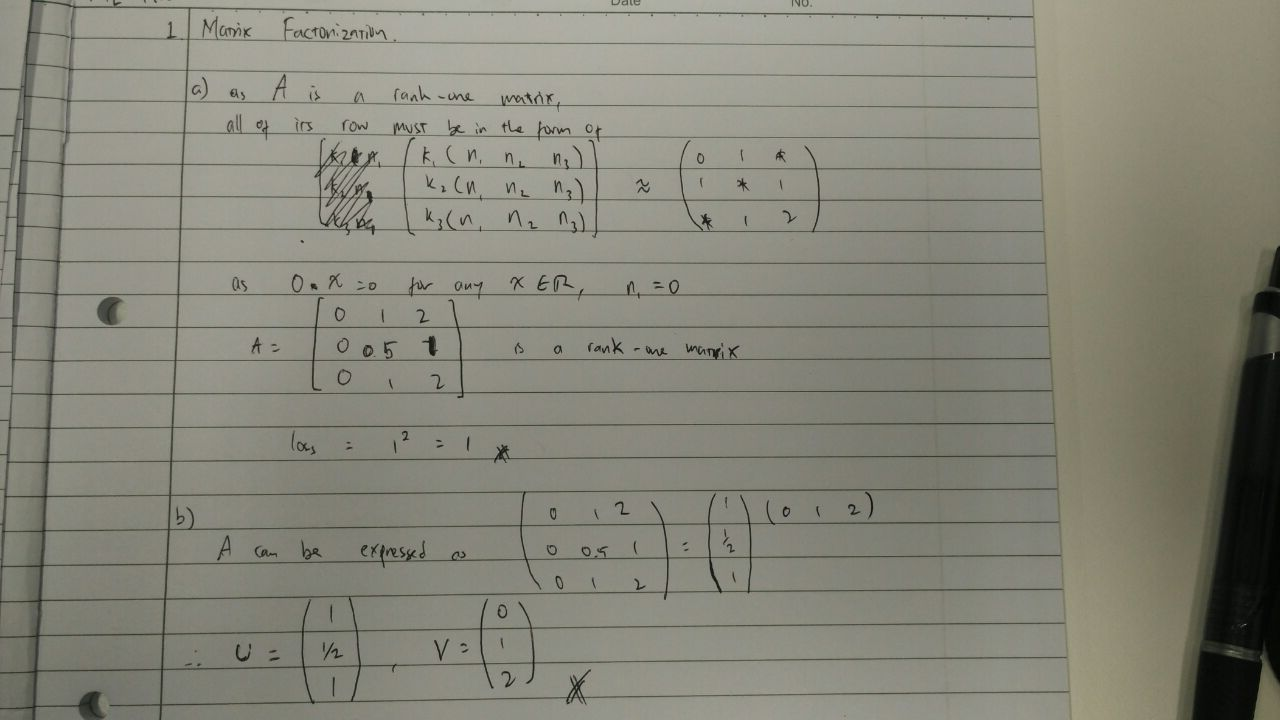
\includegraphics{factor.jpeg}
\caption{pic}
\end{figure}

    \subsubsection{Q2. Support Vector
Machines}\label{q2.-support-vector-machines}

    \begin{Verbatim}[commandchars=\\\{\}]
{\color{incolor}In [{\color{incolor}1}]:} \PY{o}{\PYZpc{}}\PY{k}{matplotlib} inline
        \PY{k+kn}{import} \PY{n+nn}{numpy} \PY{k}{as} \PY{n+nn}{np}
        \PY{k+kn}{import} \PY{n+nn}{matplotlib}\PY{n+nn}{.}\PY{n+nn}{pyplot} \PY{k}{as} \PY{n+nn}{plt}
        \PY{n}{csv} \PY{o}{=} \PY{l+s+s1}{\PYZsq{}}\PY{l+s+s1}{https://www.dropbox.com/s/wt45tvn9ig3o7vu/kernel.csv?dl=1}\PY{l+s+s1}{\PYZsq{}}
        \PY{n}{data} \PY{o}{=} \PY{n}{np}\PY{o}{.}\PY{n}{genfromtxt}\PY{p}{(}\PY{n}{csv}\PY{p}{,} \PY{n}{delimiter}\PY{o}{=}\PY{l+s+s1}{\PYZsq{}}\PY{l+s+s1}{,}\PY{l+s+s1}{\PYZsq{}}\PY{p}{)}
        \PY{n}{X} \PY{o}{=} \PY{n}{data}\PY{p}{[}\PY{p}{:}\PY{p}{,}\PY{l+m+mi}{1}\PY{p}{:}\PY{p}{]}
        \PY{n}{Y} \PY{o}{=} \PY{n}{data} \PY{p}{[}\PY{p}{:}\PY{p}{,}\PY{l+m+mi}{0}\PY{p}{]}
        \PY{n}{plt}\PY{o}{.}\PY{n}{scatter}\PY{p}{(}\PY{n}{X}\PY{p}{[}\PY{p}{:}\PY{p}{,}\PY{l+m+mi}{0}\PY{p}{]}\PY{p}{,}\PY{n}{X}\PY{p}{[}\PY{p}{:}\PY{p}{,}\PY{l+m+mi}{1}\PY{p}{]}\PY{p}{,}\PY{n}{c}\PY{o}{=}\PY{n}{Y}\PY{p}{)}
        \PY{n}{plt}\PY{o}{.}\PY{n}{show}\PY{p}{(}\PY{p}{)}
\end{Verbatim}


    \begin{center}
    \adjustimage{max size={0.9\linewidth}{0.9\paperheight}}{output_4_0.png}
    \end{center}
    { \hspace*{\fill} \\}
    
    \begin{center}\rule{0.5\linewidth}{\linethickness}\end{center}

\textbf{a)} Use the \texttt{sklearn.svm.SVC} module to train a kernel
support vector machine via the radial basis kernel. Set gamma to 0.5 and
\texttt{kernel} to \texttt{rbf}.

    \begin{Verbatim}[commandchars=\\\{\}]
{\color{incolor}In [{\color{incolor}2}]:} \PY{k+kn}{from} \PY{n+nn}{sklearn}\PY{n+nn}{.}\PY{n+nn}{svm} \PY{k}{import} \PY{n}{SVC}
        \PY{n}{dis\PYZus{}svc} \PY{o}{=} \PY{n}{SVC}\PY{p}{(}\PY{n}{gamma}\PY{o}{=}\PY{l+m+mf}{0.5}\PY{p}{,} \PY{n}{kernel}\PY{o}{=}\PY{l+s+s1}{\PYZsq{}}\PY{l+s+s1}{rbf}\PY{l+s+s1}{\PYZsq{}}\PY{p}{)}
        \PY{n}{dis\PYZus{}svc}\PY{o}{.}\PY{n}{fit}\PY{p}{(}\PY{n}{X}\PY{p}{,} \PY{n}{Y}\PY{p}{)}
\end{Verbatim}


\begin{Verbatim}[commandchars=\\\{\}]
{\color{outcolor}Out[{\color{outcolor}2}]:} SVC(C=1.0, cache\_size=200, class\_weight=None, coef0=0.0,
          decision\_function\_shape='ovr', degree=3, gamma=0.5, kernel='rbf',
          max\_iter=-1, probability=False, random\_state=None, shrinking=True,
          tol=0.001, verbose=False)
\end{Verbatim}
            
    \begin{center}\rule{0.5\linewidth}{\linethickness}\end{center}

\textbf{b)} Evaluate the kernel SVM's decision function. You may use the
\texttt{decision\_function} method in \texttt{SVC}. Write a function
that takes coordinates \texttt{x1,\ x2} and the SVC object \texttt{clf},
and return the value of decision function.

    \begin{Verbatim}[commandchars=\\\{\}]
{\color{incolor}In [{\color{incolor}3}]:} \PY{n}{clf} \PY{o}{=} \PY{n}{dis\PYZus{}svc}
        
        \PY{k}{def} \PY{n+nf}{decision}\PY{p}{(}\PY{n}{x1}\PY{p}{,} \PY{n}{x2}\PY{p}{,} \PY{n}{clf}\PY{p}{)}\PY{p}{:}
            \PY{n}{x} \PY{o}{=} \PY{n}{np}\PY{o}{.}\PY{n}{array}\PY{p}{(}\PY{p}{[}\PY{p}{[}\PY{n}{x1}\PY{p}{,} \PY{n}{x2}\PY{p}{]}\PY{p}{]}\PY{p}{)}
            \PY{n}{val} \PY{o}{=} \PY{n}{clf}\PY{o}{.}\PY{n}{decision\PYZus{}function}\PY{p}{(}\PY{n}{x}\PY{p}{)}
            \PY{k}{return} \PY{n}{val}\PY{p}{[}\PY{l+m+mi}{0}\PY{p}{]}
        
        \PY{n}{decision}\PY{p}{(}\PY{l+m+mi}{3}\PY{p}{,}\PY{l+m+mi}{5}\PY{p}{,}\PY{n}{clf}\PY{p}{)}
\end{Verbatim}


\begin{Verbatim}[commandchars=\\\{\}]
{\color{outcolor}Out[{\color{outcolor}3}]:} 1.1813851778172231
\end{Verbatim}
            
    \begin{center}\rule{0.5\linewidth}{\linethickness}\end{center}

\textbf{c)} Use the following code to visualize the classifier and the
data points.

    \begin{Verbatim}[commandchars=\\\{\}]
{\color{incolor}In [{\color{incolor}4}]:} \PY{n}{vdecision} \PY{o}{=} \PY{n}{np}\PY{o}{.}\PY{n}{vectorize}\PY{p}{(}\PY{n}{decision}\PY{p}{,}\PY{n}{excluded}\PY{o}{=}\PY{p}{[}\PY{l+m+mi}{2}\PY{p}{]}\PY{p}{)}
        \PY{n}{x1list} \PY{o}{=} \PY{n}{np}\PY{o}{.}\PY{n}{linspace}\PY{p}{(}\PY{o}{\PYZhy{}}\PY{l+m+mf}{8.0}\PY{p}{,} \PY{l+m+mf}{8.0}\PY{p}{,} \PY{l+m+mi}{100}\PY{p}{)}
        \PY{n}{x2list} \PY{o}{=} \PY{n}{np}\PY{o}{.}\PY{n}{linspace}\PY{p}{(}\PY{o}{\PYZhy{}}\PY{l+m+mf}{8.0}\PY{p}{,} \PY{l+m+mf}{8.0}\PY{p}{,} \PY{l+m+mi}{100}\PY{p}{)}
        \PY{n}{X1}\PY{p}{,} \PY{n}{X2} \PY{o}{=} \PY{n}{np}\PY{o}{.}\PY{n}{meshgrid}\PY{p}{(}\PY{n}{x1list}\PY{p}{,} \PY{n}{x2list}\PY{p}{)}
        \PY{n}{Z} \PY{o}{=} \PY{n}{vdecision}\PY{p}{(}\PY{n}{X1}\PY{p}{,} \PY{n}{X2}\PY{p}{,} \PY{n}{clf}\PY{p}{)}
        \PY{n}{cp} \PY{o}{=} \PY{n}{plt}\PY{o}{.}\PY{n}{contourf}\PY{p}{(}\PY{n}{X1}\PY{p}{,} \PY{n}{X2}\PY{p}{,} \PY{n}{Z}\PY{p}{)}
        \PY{n}{plt}\PY{o}{.}\PY{n}{colorbar}\PY{p}{(}\PY{n}{cp}\PY{p}{)}
        \PY{n}{plt}\PY{o}{.}\PY{n}{scatter}\PY{p}{(}\PY{n}{X}\PY{p}{[}\PY{p}{:}\PY{p}{,}\PY{l+m+mi}{0}\PY{p}{]}\PY{p}{,} \PY{n}{X}\PY{p}{[}\PY{p}{:}\PY{p}{,}\PY{l+m+mi}{1}\PY{p}{]}\PY{p}{,} \PY{n}{c}\PY{o}{=}\PY{n}{Y}\PY{p}{,} \PY{n}{cmap}\PY{o}{=}\PY{l+s+s1}{\PYZsq{}}\PY{l+s+s1}{gray}\PY{l+s+s1}{\PYZsq{}}\PY{p}{)}
        \PY{n}{plt}\PY{o}{.}\PY{n}{show}\PY{p}{(}\PY{p}{)}
\end{Verbatim}


    \begin{center}
    \adjustimage{max size={0.9\linewidth}{0.9\paperheight}}{output_10_0.png}
    \end{center}
    { \hspace*{\fill} \\}
    
    \subsubsection{Q3. Deep Learning}\label{q3.-deep-learning}

    \begin{Verbatim}[commandchars=\\\{\}]
{\color{incolor}In [{\color{incolor}5}]:} \PY{o}{\PYZpc{}}\PY{k}{matplotlib} inline
        \PY{k+kn}{import} \PY{n+nn}{numpy} \PY{k}{as} \PY{n+nn}{np}
        \PY{k+kn}{from} \PY{n+nn}{numpy}\PY{n+nn}{.}\PY{n+nn}{linalg} \PY{k}{import} \PY{n}{norm}
        \PY{k+kn}{import} \PY{n+nn}{matplotlib}\PY{n+nn}{.}\PY{n+nn}{pyplot} \PY{k}{as} \PY{n+nn}{plt}
        \PY{k+kn}{from} \PY{n+nn}{scipy}\PY{n+nn}{.}\PY{n+nn}{optimize} \PY{k}{import} \PY{n}{fmin\PYZus{}l\PYZus{}bfgs\PYZus{}b} \PY{k}{as} \PY{n}{minimize}
        
        \PY{k+kn}{from} \PY{n+nn}{utils} \PY{k}{import} \PY{n}{normalize}\PY{p}{,} \PY{n}{tile\PYZus{}raster\PYZus{}images}\PY{p}{,} \PY{n}{sigmoid}
        \PY{k+kn}{from} \PY{n+nn}{utils} \PY{k}{import} \PY{n}{ravelParameters}\PY{p}{,} \PY{n}{unravelParameters}
        \PY{k+kn}{from} \PY{n+nn}{utils} \PY{k}{import} \PY{n}{initializeParameters}
        \PY{k+kn}{from} \PY{n+nn}{utils} \PY{k}{import} \PY{n}{computeNumericalGradient}
\end{Verbatim}


    \begin{Verbatim}[commandchars=\\\{\}]
{\color{incolor}In [{\color{incolor}6}]:} \PY{n}{nV} \PY{o}{=} \PY{l+m+mi}{8}\PY{o}{*}\PY{l+m+mi}{8}
        \PY{n}{nH} \PY{o}{=} \PY{l+m+mi}{25}
        \PY{n}{dW} \PY{o}{=} \PY{l+m+mf}{0.0001}
        \PY{n}{sW} \PY{o}{=} \PY{l+m+mi}{3}
\end{Verbatim}


    \begin{Verbatim}[commandchars=\\\{\}]
{\color{incolor}In [{\color{incolor}7}]:} \PY{n}{npy} \PY{o}{=} \PY{l+s+s1}{\PYZsq{}}\PY{l+s+s1}{images.npy}\PY{l+s+s1}{\PYZsq{}}
        \PY{n}{X} \PY{o}{=} \PY{n}{normalize}\PY{p}{(}\PY{n}{np}\PY{o}{.}\PY{n}{load}\PY{p}{(}\PY{n}{npy}\PY{p}{)}\PY{p}{)}
        \PY{n}{plt}\PY{o}{.}\PY{n}{imshow}\PY{p}{(}\PY{n}{tile\PYZus{}raster\PYZus{}images}\PY{p}{(}\PY{n}{X}\PY{o}{=}\PY{n}{X}\PY{p}{,} \PY{n}{img\PYZus{}shape}\PY{o}{=}\PY{p}{(}\PY{l+m+mi}{8}\PY{p}{,}\PY{l+m+mi}{8}\PY{p}{)}\PY{p}{,} \PY{n}{tile\PYZus{}shape}\PY{o}{=}\PY{p}{(}\PY{l+m+mi}{5}\PY{p}{,}\PY{l+m+mi}{5}\PY{p}{)}\PY{p}{,} 
                                      \PY{n}{tile\PYZus{}spacing}\PY{o}{=}\PY{p}{(}\PY{l+m+mi}{1}\PY{p}{,}\PY{l+m+mi}{1}\PY{p}{)}\PY{p}{)}\PY{p}{,}
                   \PY{n}{cmap}\PY{o}{=}\PY{l+s+s1}{\PYZsq{}}\PY{l+s+s1}{gray}\PY{l+s+s1}{\PYZsq{}}\PY{p}{)}
        \PY{n}{plt}\PY{o}{.}\PY{n}{show}\PY{p}{(}\PY{p}{)}
\end{Verbatim}


    \begin{center}
    \adjustimage{max size={0.9\linewidth}{0.9\paperheight}}{output_14_0.png}
    \end{center}
    { \hspace*{\fill} \\}
    
    \begin{center}\rule{0.5\linewidth}{\linethickness}\end{center}

\textbf{a)} We implement the function which computes the cost and the
gradient of the sparse autoencoder. This function will be passed to an
optimization engine, together with the \texttt{theta} vector that
contains the current state of all the model parameters. The first step
of the function is therefore to unpack the \texttt{theta} vector into
\emph{W1, W2, b1, b2}.

    \begin{Verbatim}[commandchars=\\\{\}]
{\color{incolor}In [{\color{incolor}8}]:} \PY{k}{def} \PY{n+nf}{sparseAutoencoderCost}\PY{p}{(}\PY{n}{theta}\PY{p}{,} \PY{n}{nV}\PY{p}{,} \PY{n}{nH}\PY{p}{,} \PY{n}{dW}\PY{p}{,} \PY{n}{sW}\PY{p}{,} \PY{n}{X}\PY{p}{)}\PY{p}{:}
            \PY{n}{W1}\PY{p}{,} \PY{n}{W2}\PY{p}{,} \PY{n}{b1}\PY{p}{,} \PY{n}{b2} \PY{o}{=} \PY{n}{unravelParameters}\PY{p}{(}\PY{n}{theta}\PY{p}{,} \PY{n}{nH}\PY{p}{,} \PY{n}{nV}\PY{p}{)}
            \PY{n}{n} \PY{o}{=} \PY{n}{X}\PY{o}{.}\PY{n}{shape}\PY{p}{[}\PY{l+m+mi}{0}\PY{p}{]}
            
            \PY{n}{z2} \PY{o}{=} \PY{n}{np}\PY{o}{.}\PY{n}{dot}\PY{p}{(}\PY{n}{X}\PY{p}{,}\PY{n}{W1}\PY{p}{)} \PY{o}{+} \PY{n}{np}\PY{o}{.}\PY{n}{dot}\PY{p}{(}\PY{n}{np}\PY{o}{.}\PY{n}{ones}\PY{p}{(}\PY{p}{(}\PY{n}{n}\PY{p}{,}\PY{l+m+mi}{1}\PY{p}{)}\PY{p}{)}\PY{p}{,}\PY{n}{b1}\PY{o}{.}\PY{n}{T}\PY{p}{)}
            \PY{n}{a2} \PY{o}{=} \PY{n}{sigmoid}\PY{p}{(}\PY{n}{z2}\PY{p}{)}
            \PY{n}{z3} \PY{o}{=} \PY{n}{np}\PY{o}{.}\PY{n}{dot}\PY{p}{(}\PY{n}{a2}\PY{p}{,}\PY{n}{W2}\PY{p}{)} \PY{o}{+} \PY{n}{np}\PY{o}{.}\PY{n}{dot}\PY{p}{(}\PY{n}{np}\PY{o}{.}\PY{n}{ones}\PY{p}{(}\PY{p}{(}\PY{n}{n}\PY{p}{,}\PY{l+m+mi}{1}\PY{p}{)}\PY{p}{)}\PY{p}{,}\PY{n}{b2}\PY{o}{.}\PY{n}{T}\PY{p}{)}
            \PY{n}{a3} \PY{o}{=} \PY{n}{sigmoid}\PY{p}{(}\PY{n}{z3}\PY{p}{)}
            
            \PY{n}{eps} \PY{o}{=} \PY{n}{a3}\PY{o}{\PYZhy{}}\PY{n}{X}
            \PY{n}{loss} \PY{o}{=} \PY{n}{norm}\PY{p}{(}\PY{n}{eps}\PY{p}{)}\PY{o}{*}\PY{o}{*}\PY{l+m+mi}{2}\PY{o}{/}\PY{p}{(}\PY{l+m+mi}{2}\PY{o}{*}\PY{n}{n}\PY{p}{)}
            \PY{n}{decay} \PY{o}{=} \PY{l+m+mf}{0.5}\PY{o}{*}\PY{p}{(}\PY{n}{norm}\PY{p}{(}\PY{n}{W1}\PY{p}{)}\PY{o}{*}\PY{o}{*}\PY{l+m+mi}{2}\PY{o}{+}\PY{n}{norm}\PY{p}{(}\PY{n}{W2}\PY{p}{)}\PY{o}{*}\PY{o}{*}\PY{l+m+mi}{2}\PY{p}{)}
            
            \PY{c+c1}{\PYZsh{}compute sparsity terms and total cost}
            \PY{n}{rho} \PY{o}{=} \PY{l+m+mf}{0.01}
            \PY{n}{a2mean} \PY{o}{=} \PY{n}{np}\PY{o}{.}\PY{n}{mean}\PY{p}{(}\PY{n}{a2}\PY{p}{,} \PY{n}{axis}\PY{o}{=}\PY{l+m+mi}{0}\PY{p}{)}\PY{o}{.}\PY{n}{reshape}\PY{p}{(}\PY{n}{nH}\PY{p}{,} \PY{l+m+mi}{1}\PY{p}{)}
            \PY{n}{kl\PYZus{}first} \PY{o}{=} \PY{n}{rho}\PY{o}{*}\PY{n}{np}\PY{o}{.}\PY{n}{log}\PY{p}{(}\PY{n}{rho}\PY{o}{/}\PY{n}{a2mean}\PY{p}{)}
            \PY{n}{kl\PYZus{}last} \PY{o}{=} \PY{p}{(}\PY{l+m+mi}{1}\PY{o}{\PYZhy{}}\PY{n}{rho}\PY{p}{)}\PY{o}{*}\PY{n}{np}\PY{o}{.}\PY{n}{log}\PY{p}{(}\PY{p}{(}\PY{l+m+mi}{1}\PY{o}{\PYZhy{}}\PY{n}{rho}\PY{p}{)}\PY{o}{/}\PY{p}{(}\PY{l+m+mi}{1}\PY{o}{\PYZhy{}}\PY{n}{a2mean}\PY{p}{)}\PY{p}{)}
            \PY{n}{kl} \PY{o}{=} \PY{n}{np}\PY{o}{.}\PY{n}{sum}\PY{p}{(}\PY{n}{kl\PYZus{}first} \PY{o}{+} \PY{n}{kl\PYZus{}last}\PY{p}{)}
            \PY{n}{dkl} \PY{o}{=} \PY{o}{\PYZhy{}}\PY{n}{rho}\PY{o}{/}\PY{n}{a2mean}\PY{o}{+}\PY{p}{(}\PY{l+m+mi}{1}\PY{o}{\PYZhy{}}\PY{n}{rho}\PY{p}{)}\PY{o}{/}\PY{p}{(}\PY{l+m+mi}{1}\PY{o}{\PYZhy{}}\PY{n}{a2mean}\PY{p}{)}
            \PY{n}{cost} \PY{o}{=} \PY{n}{loss}\PY{o}{+}\PY{n}{dW}\PY{o}{*}\PY{n}{decay}\PY{o}{+}\PY{n}{sW}\PY{o}{*}\PY{n}{kl}
            
            \PY{n}{d3} \PY{o}{=} \PY{n}{eps}\PY{o}{*}\PY{n}{a3}\PY{o}{*}\PY{p}{(}\PY{l+m+mi}{1}\PY{o}{\PYZhy{}}\PY{n}{a3}\PY{p}{)}
            \PY{n}{d2} \PY{o}{=} \PY{p}{(}\PY{n}{sW}\PY{o}{*}\PY{n}{dkl}\PY{o}{.}\PY{n}{T}\PY{o}{+}\PY{n}{np}\PY{o}{.}\PY{n}{dot}\PY{p}{(}\PY{n}{d3}\PY{p}{,} \PY{n}{W2}\PY{o}{.}\PY{n}{T}\PY{p}{)}\PY{p}{)}\PY{o}{*}\PY{n}{a2}\PY{o}{*}\PY{p}{(}\PY{l+m+mi}{1}\PY{o}{\PYZhy{}}\PY{n}{a2}\PY{p}{)}
            \PY{n}{W1grad} \PY{o}{=} \PY{n}{np}\PY{o}{.}\PY{n}{dot}\PY{p}{(}\PY{n}{X}\PY{o}{.}\PY{n}{T}\PY{p}{,}\PY{n}{d2}\PY{p}{)}\PY{o}{/}\PY{n}{n} \PY{o}{+} \PY{n}{dW}\PY{o}{*}\PY{n}{W1}
            \PY{n}{W2grad} \PY{o}{=} \PY{n}{np}\PY{o}{.}\PY{n}{dot}\PY{p}{(}\PY{n}{a2}\PY{o}{.}\PY{n}{T}\PY{p}{,}\PY{n}{d3}\PY{p}{)}\PY{o}{/}\PY{n}{n} \PY{o}{+} \PY{n}{dW}\PY{o}{*}\PY{n}{W2}
            \PY{n}{b1grad} \PY{o}{=} \PY{n}{np}\PY{o}{.}\PY{n}{dot}\PY{p}{(}\PY{n}{d2}\PY{o}{.}\PY{n}{T}\PY{p}{,}\PY{n}{np}\PY{o}{.}\PY{n}{ones}\PY{p}{(}\PY{p}{(}\PY{n}{n}\PY{p}{,}\PY{l+m+mi}{1}\PY{p}{)}\PY{p}{)}\PY{p}{)}\PY{o}{/}\PY{n}{n}
            \PY{n}{b2grad} \PY{o}{=} \PY{n}{np}\PY{o}{.}\PY{n}{dot}\PY{p}{(}\PY{n}{d3}\PY{o}{.}\PY{n}{T}\PY{p}{,}\PY{n}{np}\PY{o}{.}\PY{n}{ones}\PY{p}{(}\PY{p}{(}\PY{n}{n}\PY{p}{,}\PY{l+m+mi}{1}\PY{p}{)}\PY{p}{)}\PY{p}{)}\PY{o}{/}\PY{n}{n}
            
            \PY{n}{grad} \PY{o}{=} \PY{n}{ravelParameters}\PY{p}{(}\PY{n}{W1grad}\PY{p}{,}\PY{n}{W2grad}\PY{p}{,}
                                   \PY{n}{b1grad}\PY{p}{,} \PY{n}{b2grad}\PY{p}{)}
            \PY{n+nb}{print}\PY{p}{(}\PY{l+s+s1}{\PYZsq{}}\PY{l+s+s1}{ .}\PY{l+s+s1}{\PYZsq{}}\PY{p}{,}\PY{n}{end}\PY{o}{=}\PY{l+s+s2}{\PYZdq{}}\PY{l+s+s2}{\PYZdq{}}\PY{p}{)}
            \PY{k}{return} \PY{n}{cost}\PY{p}{,} \PY{n}{grad}
\end{Verbatim}


    \begin{Verbatim}[commandchars=\\\{\}]
{\color{incolor}In [{\color{incolor}9}]:} \PY{n}{theta} \PY{o}{=} \PY{n}{initializeParameters}\PY{p}{(}\PY{n}{nH}\PY{p}{,} \PY{n}{nV}\PY{p}{)}
        \PY{n}{cost}\PY{p}{,} \PY{n}{grad} \PY{o}{=} \PY{n}{sparseAutoencoderCost}\PY{p}{(}\PY{n}{theta}\PY{p}{,} \PY{n}{nV}\PY{p}{,} \PY{n}{nH}\PY{p}{,} \PY{n}{dW}\PY{p}{,} \PY{n}{sW}\PY{p}{,} \PY{n}{X}\PY{p}{)}
        \PY{n+nb}{print}\PY{p}{(}\PY{n}{cost}\PY{p}{,}\PY{n}{grad}\PY{p}{)}
        \PY{c+c1}{\PYZsh{}print(np.ones(50))}
\end{Verbatim}


    \begin{Verbatim}[commandchars=\\\{\}]
 .56.5319053844 [ 0.83106574  0.87429827  0.80847634 {\ldots}, -0.02399919 -0.03810212
 -0.00833089]

    \end{Verbatim}

    \begin{center}\rule{0.5\linewidth}{\linethickness}\end{center}

\textbf{b)} Compare the backdrop gradient in
\texttt{sparseAutoencoderCost} with the gradient computed numerically
from the cost. The relative difference should be less than 10e-9.

    \begin{Verbatim}[commandchars=\\\{\}]
{\color{incolor}In [{\color{incolor}10}]:} \PY{n+nb}{print}\PY{p}{(}\PY{l+s+s1}{\PYZsq{}}\PY{l+s+se}{\PYZbs{}n}\PY{l+s+s1}{Comparing numerical gradient with backdrop gradient}\PY{l+s+s1}{\PYZsq{}}\PY{p}{)}
         \PY{n}{num\PYZus{}coords} \PY{o}{=} \PY{l+m+mi}{5}
         \PY{n}{indices} \PY{o}{=} \PY{n}{np}\PY{o}{.}\PY{n}{random}\PY{o}{.}\PY{n}{choice}\PY{p}{(}\PY{n}{theta}\PY{o}{.}\PY{n}{size}\PY{p}{,} \PY{n}{num\PYZus{}coords}\PY{p}{,} \PY{n}{replace}\PY{o}{=}\PY{k+kc}{False}\PY{p}{)}
         \PY{n}{numgrad} \PY{o}{=} \PY{n}{computeNumericalGradient}\PY{p}{(}\PY{k}{lambda} \PY{n}{t}\PY{p}{:} 
                                                \PY{n}{sparseAutoencoderCost}\PY{p}{(}\PY{n}{t}\PY{p}{,}\PY{n}{nV}\PY{p}{,}\PY{n}{nH}\PY{p}{,}\PY{n}{dW}\PY{p}{,}\PY{n}{sW}\PY{p}{,}\PY{n}{X}\PY{p}{)}\PY{p}{[}\PY{l+m+mi}{0}\PY{p}{]}\PY{p}{,}
                                            \PY{n}{theta}\PY{p}{,}\PY{n}{indices}\PY{p}{)}
         \PY{n}{subnumgrad} \PY{o}{=} \PY{n}{numgrad}\PY{p}{[}\PY{n}{indices}\PY{p}{]}
         \PY{n}{subgrad} \PY{o}{=} \PY{n}{grad}\PY{p}{[}\PY{n}{indices}\PY{p}{]}
         \PY{n}{diff} \PY{o}{=} \PY{n}{norm}\PY{p}{(}\PY{n}{subnumgrad}\PY{o}{\PYZhy{}}\PY{n}{subgrad}\PY{p}{)}\PY{o}{/}\PY{n}{norm}\PY{p}{(}\PY{n}{subnumgrad}\PY{o}{+}\PY{n}{subgrad}\PY{p}{)}
         \PY{n+nb}{print}\PY{p}{(}\PY{l+s+s1}{\PYZsq{}}\PY{l+s+se}{\PYZbs{}n}\PY{l+s+s1}{\PYZsq{}}\PY{p}{,}\PY{n}{np}\PY{o}{.}\PY{n}{array}\PY{p}{(}\PY{p}{[}\PY{n}{subnumgrad}\PY{p}{,}\PY{n}{subgrad}\PY{p}{]}\PY{p}{)}\PY{o}{.}\PY{n}{T}\PY{p}{)}
         \PY{n+nb}{print}\PY{p}{(}\PY{l+s+s1}{\PYZsq{}}\PY{l+s+s1}{Relative difference: }\PY{l+s+s1}{\PYZsq{}}\PY{p}{,} \PY{n}{diff}\PY{p}{)}
         
         \PY{k}{if} \PY{n}{diff} \PY{o}{\PYZlt{}} \PY{l+m+mi}{10}\PY{o}{*}\PY{o}{*}\PY{p}{(}\PY{o}{\PYZhy{}}\PY{l+m+mi}{9}\PY{p}{)}\PY{p}{:}
             \PY{n+nb}{print}\PY{p}{(}\PY{l+s+s2}{\PYZdq{}}\PY{l+s+s2}{small enough!}\PY{l+s+s2}{\PYZdq{}}\PY{p}{)}
         \PY{k}{else}\PY{p}{:}
             \PY{n+nb}{print}\PY{p}{(}\PY{l+s+s2}{\PYZdq{}}\PY{l+s+s2}{NOOOOO!!}\PY{l+s+s2}{\PYZdq{}}\PY{p}{)}
\end{Verbatim}


    \begin{Verbatim}[commandchars=\\\{\}]

Comparing numerical gradient with backdrop gradient
 . . . . . . . . . .
 [[ -5.60882391e-03  -5.60882395e-03]
 [  8.31224652e-01   8.31224652e-01]
 [ -4.60600091e-05  -4.60599727e-05]
 [  1.60391841e-02   1.60391841e-02]
 [  5.93707750e-01   5.93707750e-01]]
Relative difference:  9.6956630679e-11
small enough!

    \end{Verbatim}

    \begin{center}\rule{0.5\linewidth}{\linethickness}\end{center}

\textbf{c)} Finally, run the following code to train the deep neural
network and to visualize the features learnt by the autoencoder. The
optimization takes several minutes.

    \begin{Verbatim}[commandchars=\\\{\}]
{\color{incolor}In [{\color{incolor}11}]:} \PY{n+nb}{print}\PY{p}{(}\PY{l+s+s1}{\PYZsq{}}\PY{l+s+se}{\PYZbs{}n}\PY{l+s+s1}{Training neural network}\PY{l+s+s1}{\PYZsq{}}\PY{p}{)}
         \PY{n}{theta} \PY{o}{=} \PY{n}{initializeParameters}\PY{p}{(}\PY{n}{nH}\PY{p}{,}\PY{n}{nV}\PY{p}{)}
         \PY{n}{opttheta}\PY{p}{,}\PY{n}{cost}\PY{p}{,}\PY{n}{msg} \PY{o}{=} \PY{n}{minimize}\PY{p}{(}\PY{n}{sparseAutoencoderCost}\PY{p}{,}
                                      \PY{n}{theta}\PY{p}{,}\PY{n}{fprime}\PY{o}{=}\PY{k+kc}{None}\PY{p}{,}\PY{n}{maxiter}\PY{o}{=}\PY{l+m+mi}{400}\PY{p}{,}
                                      \PY{n}{args}\PY{o}{=}\PY{p}{(}\PY{n}{nV}\PY{p}{,}\PY{n}{nH}\PY{p}{,}\PY{n}{dW}\PY{p}{,}\PY{n}{sW}\PY{p}{,}\PY{n}{X}\PY{p}{)}\PY{p}{)}
         \PY{n}{W1}\PY{p}{,}\PY{n}{W2}\PY{p}{,}\PY{n}{b1}\PY{p}{,}\PY{n}{b2} \PY{o}{=} \PY{n}{unravelParameters}\PY{p}{(}\PY{n}{opttheta}\PY{p}{,}\PY{n}{nH}\PY{p}{,}\PY{n}{nV}\PY{p}{)}
         \PY{n}{plt}\PY{o}{.}\PY{n}{imshow}\PY{p}{(}\PY{n}{tile\PYZus{}raster\PYZus{}images}\PY{p}{(}\PY{n}{X}\PY{o}{=}\PY{n}{W1}\PY{o}{.}\PY{n}{T}\PY{p}{,} \PY{n}{img\PYZus{}shape}\PY{o}{=}\PY{p}{(}\PY{l+m+mi}{8}\PY{p}{,}\PY{l+m+mi}{8}\PY{p}{)}\PY{p}{,}
                                       \PY{n}{tile\PYZus{}shape}\PY{o}{=}\PY{p}{(}\PY{l+m+mi}{5}\PY{p}{,}\PY{l+m+mi}{5}\PY{p}{)}\PY{p}{,}\PY{n}{tile\PYZus{}spacing}\PY{o}{=}\PY{p}{(}\PY{l+m+mi}{1}\PY{p}{,}\PY{l+m+mi}{1}\PY{p}{)}\PY{p}{)}\PY{p}{,}
                    \PY{n}{cmap}\PY{o}{=}\PY{l+s+s1}{\PYZsq{}}\PY{l+s+s1}{gray}\PY{l+s+s1}{\PYZsq{}}\PY{p}{)}
         \PY{n}{plt}\PY{o}{.}\PY{n}{show}\PY{p}{(}\PY{p}{)}
\end{Verbatim}


    \begin{Verbatim}[commandchars=\\\{\}]

Training neural network
 . . . . . . . . . . . . . . . . . . . . . . . . . . . . . . . . . . . . . . . . . . . . . . . . . . . . . . . . . . . . . . . . . . . . . . . . . . . . . . . . . . . . . . . . . . . . . . . . . . . . . . . . . . . . . . . . . . . . . . . . . . . . . . . . . . . . . . . . . . . . . . . . . . . . . . . . . . . . . . . . . . . . . . . . . . . . . . . . . . . . . . . . . . . . . . . . . . . . . . . . . . . . . . . . . . . . . . . . . . . . . . . . . . . . . . . . . . . . . . . . . . . . . . . . . . . . . . . . . . . . . . . . . . . . . . . . . . . . . . . . . . . . . . . . . . . . . . . . . . . . . . . . . . . . . . . . . . . . . . . . . . . . . . . . . . . . . . . . . . . . . . . . . . . . . . . . . . . . . . . . . . . . . . . . . . . . . . . . . . . . . . . . . . . . . . . . . . . . . . . . . . . . . . . . . . . . . . . . . .
    \end{Verbatim}

    \begin{center}
    \adjustimage{max size={0.9\linewidth}{0.9\paperheight}}{output_21_1.png}
    \end{center}
    { \hspace*{\fill} \\}
    
    \subsubsection{Q4. DataSpark Challenge}\label{q4.-dataspark-challenge}

    \begin{Verbatim}[commandchars=\\\{\}]
{\color{incolor}In [{\color{incolor}12}]:} \PY{o}{\PYZpc{}}\PY{k}{matplotlib} inline
         \PY{k+kn}{import} \PY{n+nn}{numpy} \PY{k}{as} \PY{n+nn}{np}
         \PY{k+kn}{import} \PY{n+nn}{pandas} \PY{k}{as} \PY{n+nn}{pd}
         \PY{k+kn}{import} \PY{n+nn}{matplotlib}\PY{n+nn}{.}\PY{n+nn}{pyplot} \PY{k}{as} \PY{n+nn}{plt}
         \PY{k+kn}{from} \PY{n+nn}{IPython}\PY{n+nn}{.}\PY{n+nn}{display} \PY{k}{import} \PY{n}{display}
\end{Verbatim}


    \begin{Verbatim}[commandchars=\\\{\}]
{\color{incolor}In [{\color{incolor}13}]:} \PY{n}{data} \PY{o}{=} \PY{n}{pd}\PY{o}{.}\PY{n}{read\PYZus{}csv}\PY{p}{(}\PY{l+s+s1}{\PYZsq{}}\PY{l+s+s1}{dataspark.csv}\PY{l+s+s1}{\PYZsq{}}\PY{p}{)}
         \PY{n}{data} \PY{o}{=} \PY{n}{data}\PY{o}{.}\PY{n}{drop}\PY{p}{(}\PY{p}{[}\PY{l+s+s1}{\PYZsq{}}\PY{l+s+s1}{seqid}\PY{l+s+s1}{\PYZsq{}}\PY{p}{,}\PY{l+s+s1}{\PYZsq{}}\PY{l+s+s1}{index}\PY{l+s+s1}{\PYZsq{}}\PY{p}{,}\PY{l+s+s1}{\PYZsq{}}\PY{l+s+s1}{acc}\PY{l+s+s1}{\PYZsq{}}\PY{p}{,}\PY{l+s+s1}{\PYZsq{}}\PY{l+s+s1}{dir}\PY{l+s+s1}{\PYZsq{}}\PY{p}{,}\PY{l+s+s1}{\PYZsq{}}\PY{l+s+s1}{spd}\PY{l+s+s1}{\PYZsq{}}\PY{p}{]}\PY{p}{,}
                          \PY{n}{axis}\PY{o}{=}\PY{l+m+mi}{1}\PY{p}{)}
         \PY{n+nb}{print}\PY{p}{(}\PY{n}{data}\PY{o}{.}\PY{n}{info}\PY{p}{(}\PY{p}{)}\PY{p}{)}
         \PY{n}{plt}\PY{o}{.}\PY{n}{scatter}\PY{p}{(}\PY{n}{data}\PY{p}{[}\PY{l+s+s1}{\PYZsq{}}\PY{l+s+s1}{lon}\PY{l+s+s1}{\PYZsq{}}\PY{p}{]}\PY{p}{,}\PY{n}{data}\PY{p}{[}\PY{l+s+s1}{\PYZsq{}}\PY{l+s+s1}{lat}\PY{l+s+s1}{\PYZsq{}}\PY{p}{]}\PY{p}{,}\PY{n}{marker}\PY{o}{=}\PY{l+s+s1}{\PYZsq{}}\PY{l+s+s1}{.}\PY{l+s+s1}{\PYZsq{}}\PY{p}{)}
         \PY{n}{plt}\PY{o}{.}\PY{n}{show}\PY{p}{(}\PY{p}{)}
         \PY{c+c1}{\PYZsh{}data = data.sample(frac=0.05, random\PYZus{}state=200)}
\end{Verbatim}


    \begin{Verbatim}[commandchars=\\\{\}]
<class 'pandas.core.frame.DataFrame'>
RangeIndex: 141437 entries, 0 to 141436
Data columns (total 4 columns):
date      141437 non-null object
userid    141437 non-null object
lat       141437 non-null float64
lon       141437 non-null float64
dtypes: float64(2), object(2)
memory usage: 4.3+ MB
None

    \end{Verbatim}

    \begin{center}
    \adjustimage{max size={0.9\linewidth}{0.9\paperheight}}{output_24_1.png}
    \end{center}
    { \hspace*{\fill} \\}
    
    \begin{Verbatim}[commandchars=\\\{\}]
{\color{incolor}In [{\color{incolor}14}]:} \PY{n}{data}\PY{p}{[}\PY{l+s+s1}{\PYZsq{}}\PY{l+s+s1}{date}\PY{l+s+s1}{\PYZsq{}}\PY{p}{]} \PY{o}{=} \PY{n}{pd}\PY{o}{.}\PY{n}{DatetimeIndex}\PY{p}{(}\PY{n}{data}\PY{p}{[}\PY{l+s+s1}{\PYZsq{}}\PY{l+s+s1}{date}\PY{l+s+s1}{\PYZsq{}}\PY{p}{]}\PY{p}{)}\PY{o}{.}\PY{n}{round}\PY{p}{(}\PY{l+s+s1}{\PYZsq{}}\PY{l+s+s1}{5min}\PY{l+s+s1}{\PYZsq{}}\PY{p}{)}
         \PY{n}{data} \PY{o}{=} \PY{n}{data}\PY{o}{.}\PY{n}{groupby}\PY{p}{(}\PY{p}{[}\PY{l+s+s1}{\PYZsq{}}\PY{l+s+s1}{userid}\PY{l+s+s1}{\PYZsq{}}\PY{p}{,}\PY{l+s+s1}{\PYZsq{}}\PY{l+s+s1}{date}\PY{l+s+s1}{\PYZsq{}}\PY{p}{]}\PY{p}{)}\PY{o}{.}\PY{n}{mean}\PY{p}{(}\PY{p}{)}\PY{o}{.}\PY{n}{reset\PYZus{}index}\PY{p}{(}\PY{p}{)}
         \PY{n+nb}{print}\PY{p}{(}\PY{n}{data}\PY{o}{.}\PY{n}{info}\PY{p}{(}\PY{p}{)}\PY{p}{)}
         \PY{n}{plt}\PY{o}{.}\PY{n}{scatter}\PY{p}{(}\PY{n}{data}\PY{p}{[}\PY{l+s+s1}{\PYZsq{}}\PY{l+s+s1}{lon}\PY{l+s+s1}{\PYZsq{}}\PY{p}{]}\PY{p}{,}\PY{n}{data}\PY{p}{[}\PY{l+s+s1}{\PYZsq{}}\PY{l+s+s1}{lat}\PY{l+s+s1}{\PYZsq{}}\PY{p}{]}\PY{p}{,}\PY{n}{marker}\PY{o}{=}\PY{l+s+s1}{\PYZsq{}}\PY{l+s+s1}{.}\PY{l+s+s1}{\PYZsq{}}\PY{p}{)}
         \PY{n}{plt}\PY{o}{.}\PY{n}{show}\PY{p}{(}\PY{p}{)}
\end{Verbatim}


    \begin{Verbatim}[commandchars=\\\{\}]
<class 'pandas.core.frame.DataFrame'>
RangeIndex: 26115 entries, 0 to 26114
Data columns (total 4 columns):
userid    26115 non-null object
date      26115 non-null datetime64[ns]
lat       26115 non-null float64
lon       26115 non-null float64
dtypes: datetime64[ns](1), float64(2), object(1)
memory usage: 816.2+ KB
None

    \end{Verbatim}

    \begin{center}
    \adjustimage{max size={0.9\linewidth}{0.9\paperheight}}{output_25_1.png}
    \end{center}
    { \hspace*{\fill} \\}
    
    \begin{center}\rule{0.5\linewidth}{\linethickness}\end{center}

\textbf{a)} Cluster the GPS locations for all users to find commonly
visited places. Us the 'elbow' method to find a suitable number of
clusters. Sample the data to improve speed. Write your guess for the
number of clusters in the data.

    \begin{Verbatim}[commandchars=\\\{\}]
{\color{incolor}In [{\color{incolor}15}]:} \PY{k+kn}{from} \PY{n+nn}{sklearn}\PY{n+nn}{.}\PY{n+nn}{cluster} \PY{k}{import} \PY{n}{KMeans}
         \PY{n}{smp} \PY{o}{=} \PY{n}{data}\PY{p}{[}\PY{p}{[}\PY{l+s+s1}{\PYZsq{}}\PY{l+s+s1}{lat}\PY{l+s+s1}{\PYZsq{}}\PY{p}{,}\PY{l+s+s1}{\PYZsq{}}\PY{l+s+s1}{lon}\PY{l+s+s1}{\PYZsq{}}\PY{p}{]}\PY{p}{]}\PY{o}{.}\PY{n}{sample}\PY{p}{(}\PY{n}{n}\PY{o}{=}\PY{l+m+mi}{3000}\PY{p}{,}\PY{n}{random\PYZus{}state}\PY{o}{=}\PY{l+m+mi}{200}\PY{p}{)}
         \PY{n}{score} \PY{o}{=} \PY{p}{[}\PY{p}{]}
         \PY{n}{cls\PYZus{}range} \PY{o}{=} \PY{n+nb}{list}\PY{p}{(}\PY{n+nb}{range}\PY{p}{(}\PY{l+m+mi}{10}\PY{p}{,}\PY{l+m+mi}{150}\PY{p}{,}\PY{l+m+mi}{10}\PY{p}{)}\PY{p}{)}
         \PY{k}{for} \PY{n}{num\PYZus{}cls} \PY{o+ow}{in} \PY{n}{cls\PYZus{}range}\PY{p}{:}
             \PY{n}{n\PYZus{}cluster} \PY{o}{=} \PY{n}{KMeans}\PY{p}{(}\PY{n}{n\PYZus{}clusters}\PY{o}{=}\PY{n}{num\PYZus{}cls}\PY{p}{)}\PY{o}{.}\PY{n}{fit}\PY{p}{(}\PY{n}{smp}\PY{p}{)}
             \PY{n}{score}\PY{o}{.}\PY{n}{append}\PY{p}{(}\PY{n}{n\PYZus{}cluster}\PY{o}{.}\PY{n}{inertia\PYZus{}}\PY{p}{)}
         \PY{n}{plt}\PY{o}{.}\PY{n}{plot}\PY{p}{(}\PY{n}{cls\PYZus{}range}\PY{p}{,}\PY{n}{score}\PY{p}{)}
         \PY{n}{plt}\PY{o}{.}\PY{n}{show}\PY{p}{(}\PY{p}{)}
\end{Verbatim}


    \begin{center}
    \adjustimage{max size={0.9\linewidth}{0.9\paperheight}}{output_27_0.png}
    \end{center}
    { \hspace*{\fill} \\}
    
    My guess is that we have 80 clusters.

    \begin{center}\rule{0.5\linewidth}{\linethickness}\end{center}

\textbf{b)} Visualize the trained centroids. In the code below,
\texttt{centroid} is a numpy array where each row consists of the
latitude of some centroid.

    \begin{Verbatim}[commandchars=\\\{\}]
{\color{incolor}In [{\color{incolor}16}]:} \PY{n}{num\PYZus{}cluster} \PY{o}{=} \PY{l+m+mi}{80}
         \PY{n}{data\PYZus{}latlon} \PY{o}{=} \PY{n}{data}\PY{p}{[}\PY{p}{[}\PY{l+s+s1}{\PYZsq{}}\PY{l+s+s1}{lat}\PY{l+s+s1}{\PYZsq{}}\PY{p}{,}\PY{l+s+s1}{\PYZsq{}}\PY{l+s+s1}{lon}\PY{l+s+s1}{\PYZsq{}}\PY{p}{]}\PY{p}{]}
         \PY{n}{decided\PYZus{}kmean} \PY{o}{=} \PY{n}{KMeans}\PY{p}{(}\PY{n}{n\PYZus{}clusters}\PY{o}{=}\PY{n}{num\PYZus{}cluster}\PY{p}{)}\PY{o}{.}\PY{n}{fit}\PY{p}{(}\PY{n}{data\PYZus{}latlon}\PY{p}{)}
         \PY{n}{centroids} \PY{o}{=} \PY{n}{decided\PYZus{}kmean}\PY{o}{.}\PY{n}{cluster\PYZus{}centers\PYZus{}}
         \PY{n}{plt}\PY{o}{.}\PY{n}{scatter}\PY{p}{(}\PY{n}{centroids}\PY{p}{[}\PY{p}{:}\PY{p}{,}\PY{l+m+mi}{1}\PY{p}{]}\PY{p}{,}\PY{n}{centroids}\PY{p}{[}\PY{p}{:}\PY{p}{,}\PY{l+m+mi}{0}\PY{p}{]}\PY{p}{)}
         \PY{n}{plt}\PY{o}{.}\PY{n}{show}\PY{p}{(}\PY{p}{)}
\end{Verbatim}


    \begin{center}
    \adjustimage{max size={0.9\linewidth}{0.9\paperheight}}{output_30_0.png}
    \end{center}
    { \hspace*{\fill} \\}
    
    \begin{center}\rule{0.5\linewidth}{\linethickness}\end{center}

\textbf{c)} Compute the speeds at which each user is travelling.

    \begin{Verbatim}[commandchars=\\\{\}]
{\color{incolor}In [{\color{incolor}47}]:} \PY{k+kn}{from} \PY{n+nn}{numpy}\PY{n+nn}{.}\PY{n+nn}{linalg} \PY{k}{import} \PY{n}{norm}
         \PY{k}{for} \PY{n}{u} \PY{o+ow}{in} \PY{n}{data}\PY{p}{[}\PY{l+s+s1}{\PYZsq{}}\PY{l+s+s1}{userid}\PY{l+s+s1}{\PYZsq{}}\PY{p}{]}\PY{o}{.}\PY{n}{unique}\PY{p}{(}\PY{p}{)}\PY{p}{:}
             \PY{n}{user} \PY{o}{=} \PY{n}{data}\PY{p}{[}\PY{n}{data}\PY{p}{[}\PY{l+s+s1}{\PYZsq{}}\PY{l+s+s1}{userid}\PY{l+s+s1}{\PYZsq{}}\PY{p}{]}\PY{o}{==}\PY{n}{u}\PY{p}{]}
             \PY{n}{date} \PY{o}{=} \PY{n}{pd}\PY{o}{.}\PY{n}{DatetimeIndex}\PY{p}{(}\PY{n}{user}\PY{p}{[}\PY{l+s+s1}{\PYZsq{}}\PY{l+s+s1}{date}\PY{l+s+s1}{\PYZsq{}}\PY{p}{]}\PY{p}{)}
             \PY{n}{hour} \PY{o}{=} \PY{p}{(}\PY{n}{date}\PY{o}{\PYZhy{}}\PY{n}{date}\PY{p}{[}\PY{l+m+mi}{0}\PY{p}{]}\PY{p}{)}\PY{o}{/}\PY{n}{np}\PY{o}{.}\PY{n}{timedelta64}\PY{p}{(}\PY{l+m+mi}{1}\PY{p}{,}\PY{l+s+s1}{\PYZsq{}}\PY{l+s+s1}{h}\PY{l+s+s1}{\PYZsq{}}\PY{p}{)}
             \PY{n}{hourfor} \PY{o}{=} \PY{n}{np}\PY{o}{.}\PY{n}{append}\PY{p}{(}\PY{n}{hour}\PY{p}{[}\PY{l+m+mi}{1}\PY{p}{:}\PY{p}{]}\PY{p}{,} \PY{n}{hour}\PY{p}{[}\PY{o}{\PYZhy{}}\PY{l+m+mi}{1}\PY{p}{]}\PY{p}{)}
             \PY{n}{dur} \PY{o}{=} \PY{n}{hourfor} \PY{o}{\PYZhy{}} \PY{n}{hour}
             
             \PY{n}{latlon} \PY{o}{=} \PY{n}{user}\PY{p}{[}\PY{p}{[}\PY{l+s+s1}{\PYZsq{}}\PY{l+s+s1}{lat}\PY{l+s+s1}{\PYZsq{}}\PY{p}{,}\PY{l+s+s1}{\PYZsq{}}\PY{l+s+s1}{lon}\PY{l+s+s1}{\PYZsq{}}\PY{p}{]}\PY{p}{]}\PY{o}{.}\PY{n}{get\PYZus{}values}\PY{p}{(}\PY{p}{)}
             \PY{n}{latlonfor} \PY{o}{=} \PY{n}{np}\PY{o}{.}\PY{n}{vstack}\PY{p}{(}\PY{p}{[}\PY{n}{latlon}\PY{p}{[}\PY{l+m+mi}{1}\PY{p}{:}\PY{p}{]}\PY{p}{,}\PY{n}{latlon}\PY{p}{[}\PY{o}{\PYZhy{}}\PY{l+m+mi}{1}\PY{p}{]}\PY{p}{]}\PY{p}{)}
             \PY{n}{displacement} \PY{o}{=} \PY{p}{(}\PY{n}{latlonfor} \PY{o}{\PYZhy{}} \PY{n}{latlon}\PY{p}{)}\PY{o}{*}\PY{o}{*}\PY{l+m+mi}{2}
             \PY{n}{disp\PYZus{}p} \PY{o}{=} \PY{p}{(}\PY{n}{displacement}\PY{p}{[}\PY{p}{:}\PY{p}{,}\PY{l+m+mi}{0}\PY{p}{]} \PY{o}{+} \PY{n}{displacement}\PY{p}{[}\PY{p}{:}\PY{p}{,}\PY{l+m+mi}{1}\PY{p}{]}\PY{p}{)}\PY{o}{*}\PY{o}{*}\PY{l+m+mf}{0.5}
             
             \PY{n}{speed} \PY{o}{=} \PY{l+m+mi}{111}\PY{o}{*}\PY{n}{disp\PYZus{}p}\PY{o}{/}\PY{n}{dur}
             \PY{n}{data}\PY{o}{.}\PY{n}{loc}\PY{p}{[}\PY{n}{data}\PY{p}{[}\PY{l+s+s1}{\PYZsq{}}\PY{l+s+s1}{userid}\PY{l+s+s1}{\PYZsq{}}\PY{p}{]}\PY{o}{==}\PY{n}{u}\PY{p}{,}\PY{l+s+s1}{\PYZsq{}}\PY{l+s+s1}{speed}\PY{l+s+s1}{\PYZsq{}}\PY{p}{]} \PY{o}{=} \PY{n}{speed}
\end{Verbatim}


    \begin{Verbatim}[commandchars=\\\{\}]
{\color{incolor}In [{\color{incolor}49}]:} \PY{n}{stop} \PY{o}{=} \PY{n}{data}\PY{p}{[}\PY{n}{data}\PY{p}{[}\PY{l+s+s1}{\PYZsq{}}\PY{l+s+s1}{speed}\PY{l+s+s1}{\PYZsq{}}\PY{p}{]}\PY{o}{\PYZlt{}}\PY{l+m+mi}{1}\PY{p}{]}
         \PY{n}{plt}\PY{o}{.}\PY{n}{scatter}\PY{p}{(}\PY{n}{stop}\PY{p}{[}\PY{l+s+s1}{\PYZsq{}}\PY{l+s+s1}{lon}\PY{l+s+s1}{\PYZsq{}}\PY{p}{]}\PY{p}{,}\PY{n}{stop}\PY{p}{[}\PY{l+s+s1}{\PYZsq{}}\PY{l+s+s1}{lat}\PY{l+s+s1}{\PYZsq{}}\PY{p}{]}\PY{p}{,}
                     \PY{n}{c}\PY{o}{=}\PY{n}{np}\PY{o}{.}\PY{n}{log}\PY{p}{(}\PY{n}{stop}\PY{p}{[}\PY{l+s+s1}{\PYZsq{}}\PY{l+s+s1}{speed}\PY{l+s+s1}{\PYZsq{}}\PY{p}{]}\PY{o}{+}\PY{l+m+mi}{1}\PY{p}{)}\PY{p}{,}
                     \PY{n}{marker}\PY{o}{=}\PY{l+s+s1}{\PYZsq{}}\PY{l+s+s1}{.}\PY{l+s+s1}{\PYZsq{}}\PY{p}{)}
         \PY{n}{plt}\PY{o}{.}\PY{n}{show}\PY{p}{(}\PY{p}{)}
         \PY{n+nb}{print}\PY{p}{(}\PY{l+s+s1}{\PYZsq{}}\PY{l+s+s1}{Number of entries =}\PY{l+s+s1}{\PYZsq{}}\PY{p}{,}\PY{n}{stop}\PY{o}{.}\PY{n}{shape}\PY{p}{[}\PY{l+m+mi}{0}\PY{p}{]}\PY{p}{)}
         
         \PY{n}{move} \PY{o}{=} \PY{n}{data}\PY{p}{[}\PY{n}{data}\PY{p}{[}\PY{l+s+s1}{\PYZsq{}}\PY{l+s+s1}{speed}\PY{l+s+s1}{\PYZsq{}}\PY{p}{]}\PY{o}{\PYZgt{}}\PY{o}{=}\PY{l+m+mi}{1}\PY{p}{]}
         \PY{n}{plt}\PY{o}{.}\PY{n}{scatter}\PY{p}{(}\PY{n}{move}\PY{p}{[}\PY{l+s+s1}{\PYZsq{}}\PY{l+s+s1}{lon}\PY{l+s+s1}{\PYZsq{}}\PY{p}{]}\PY{p}{,}\PY{n}{move}\PY{p}{[}\PY{l+s+s1}{\PYZsq{}}\PY{l+s+s1}{lat}\PY{l+s+s1}{\PYZsq{}}\PY{p}{]}\PY{p}{,}
                     \PY{n}{c}\PY{o}{=}\PY{n}{np}\PY{o}{.}\PY{n}{log}\PY{p}{(}\PY{n}{move}\PY{p}{[}\PY{l+s+s1}{\PYZsq{}}\PY{l+s+s1}{speed}\PY{l+s+s1}{\PYZsq{}}\PY{p}{]}\PY{o}{+}\PY{l+m+mi}{1}\PY{p}{)}\PY{p}{,}
                     \PY{n}{marker}\PY{o}{=}\PY{l+s+s1}{\PYZsq{}}\PY{l+s+s1}{.}\PY{l+s+s1}{\PYZsq{}}\PY{p}{)}
         \PY{n}{plt}\PY{o}{.}\PY{n}{show}\PY{p}{(}\PY{p}{)}
         \PY{n+nb}{print}\PY{p}{(}\PY{l+s+s1}{\PYZsq{}}\PY{l+s+s1}{Number of entries =}\PY{l+s+s1}{\PYZsq{}}\PY{p}{,}\PY{n}{move}\PY{o}{.}\PY{n}{shape}\PY{p}{[}\PY{l+m+mi}{0}\PY{p}{]}\PY{p}{)}
\end{Verbatim}


    \begin{center}
    \adjustimage{max size={0.9\linewidth}{0.9\paperheight}}{output_33_0.png}
    \end{center}
    { \hspace*{\fill} \\}
    
    \begin{Verbatim}[commandchars=\\\{\}]
Number of entries = 20921

    \end{Verbatim}

    \begin{center}
    \adjustimage{max size={0.9\linewidth}{0.9\paperheight}}{output_33_2.png}
    \end{center}
    { \hspace*{\fill} \\}
    
    \begin{Verbatim}[commandchars=\\\{\}]
Number of entries = 5164

    \end{Verbatim}


    % Add a bibliography block to the postdoc
    
    
    
    \end{document}
